\section{Aufbau der Signalverzögerung und MOSFET-Endstufe}
In dieser Übung wird die Schaltung um drei Funktionsblöcke ergänzt: Signalverzögerung, MOSFET-Treiberstufe und MOSFET-Gegentaktendstufe. Ziel ist es, das PWM-Signal mit definierter Totzeit aufzubereiten, die MOSFETs sicher und schnell anzusteuern und am Ausgang eine leistungsfähige Endstufe bereitzustellen.

\subsection{Schaltung}
Die Schaltung \cref{fig:schaltung_endstufe} besteht aus:

\textbf{Signalverzögerung:} Das PWM-Signal wird durch NAND-Gatter in Kombination mit RC-Gliedern verzögert. Die Zeitkonstante ergibt sich aus $\tau = R \cdot C$ und beträgt mit $R=6{,}8\,k\Omega$ und $C=39\,pF$:
\[ 
  \tau = 6{,}8\,k\Omega \cdot 39\,pF \approx 2{,}65 \cdot 10^{-7}\,s \approx 265\,ns
\]
Damit wird eine Totzeit erzeugt, die ein gleichzeitiges Durchschalten der MOSFETs verhindert.

\textbf{MOSFET-Treiber:} Die verzögerten Signale werden durch mehrere CMOS-Inverter verstärkt. Diese dienen als Treiberstufe, um die MOSFETs mit ausreichend Strom anzusteuern und schnelles Schalten zu ermöglichen.

\textbf{MOSFET-Gegentakt-Endstufe:} Die verstärkten Signale steuern die Endstufe, die aus Q1 und Q2 besteht. Dadurch entsteht ein leistungsfähiges PWM-Signal am Ausgang.

\begin{figure}[H]
  \centering
  % TODO: Bildpfad einsetzen
  %\includegraphics[width=0.7\linewidth]{Signalaufbereitung/DEIN_BILDNAME}
  \caption{Schaltung der Signalverzögerung und MOSFET-Endstufe}
  \label{fig:schaltung_endstufe}
\end{figure}

\subsection{Messvorgang}
Zunächst wird die Schaltung bis einschließlich der Treiberstufe aufgebaut, um die Signalverzögerung zu verifizieren. Gemessen wird mit dem Oszilloskop an den Ausgängen der beiden MOSFET-Treiber.

\subsection{Messergebnis}
In \cref{fig:signalaufbereitungvorendstufe}, auf CH1 ist der P-Channel, auf CH2 der N-Channel zu sehen. Der P-Channel sperrt etwa $280\,ns$ vor dem Leiten des N-Channels.

\begin{figure}[h]
  \centering
  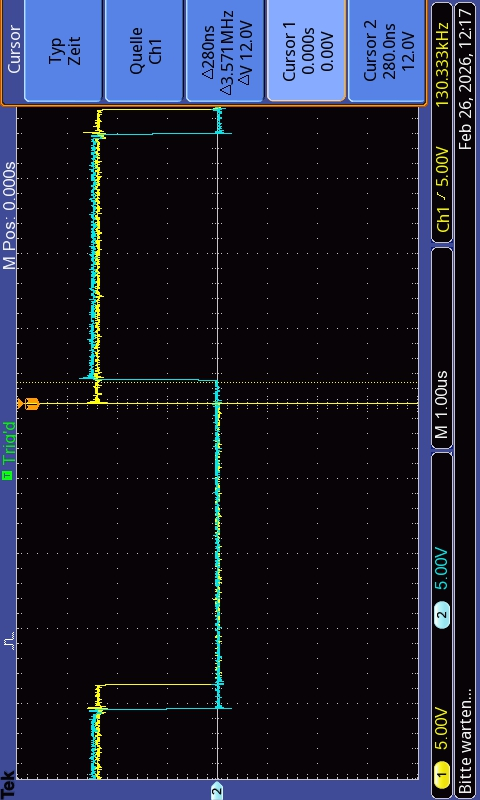
\includegraphics[width=0.4\linewidth, angle = -90]{Signalaufbereitung/SignalaufbereitungVorEndstufe}
  \caption{Messung am Ausgang der Signalaufbereitung}
  \label{fig:signalaufbereitungvorendstufe}
\end{figure}

\subsection{Interpretation}
Die berechnete Totzeit von ca. $265\,ns$ liegt sehr nahe am gemessenen Versatz von etwa $280\,ns$. Damit passt die RC-Dimensionierung zur gewünschten Signalverzögerung und verhindert zuverlässig Überschneidungen beim Schalten der MOSFETs.
